\subsection{\label{sec:A1}Autokorrelation}
Zunächst ist es erforderlich, aus der aufgezeichneten Autokorrelation die genannten interferometrischen 
Beiträge zu extrahieren, um präzisere Analysen zu ermöglichen. Hierzu werden die hochfrequenten Komponenten 
der Fouriertransformation des aufgezeichneten Signals abgeschnitten, und das zurücktransformierte Signal wird 
betrachtet. In Abbildung~\ref{fig:A11} sind die gemessene Intensitätsautokorrelationsfunktion (IAKF), 
das gefilterte Signal und das Fourier-Spektrum der IAKF dargestellt.
\begin{figure}[h!]
    \centering
    \subfloat[\centering gemessenes Signal (IAKF)]{{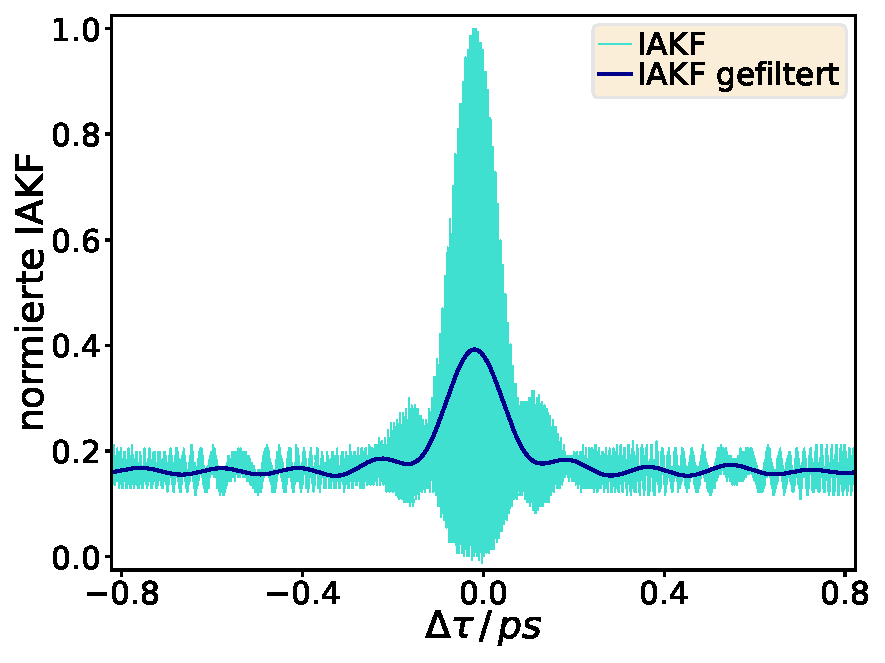
\includegraphics[width=0.47\textwidth]{IAKF.pdf} }}
    \qquad
    \subfloat[\centering Fouriertransformierte IAKF]{{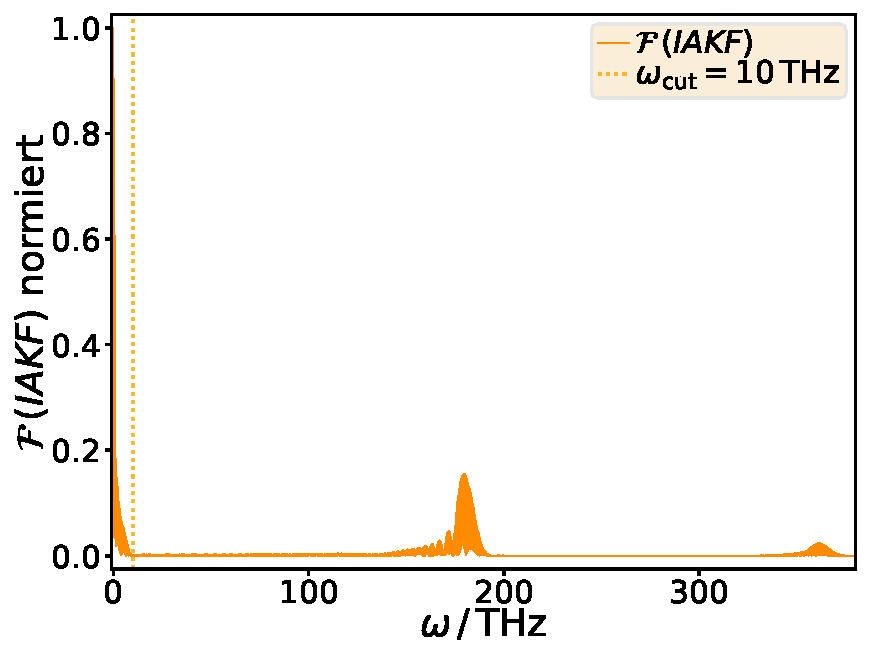
\includegraphics[width=0.47\textwidth]{FTIAKF.pdf} }}
    \caption{\label{fig:A11}a) Gemessenes Diodensignal als Funktion der zeitlichen Verzögerung $\Delta\tau$,
    sowie gefiltertes Signal. b) Fourier-Spektrum des gemessenen Signals und gewählte 
    Cutoff-Frequenz $\omega_{\text{cut}}$.}
\end{figure}\FloatBarrier
Die IAKF zeigt, wie erwartet, Symmetrie und konvergiert für $\Delta\tau \rightarrow 0$ gegen ihren Maximalwert. 
Dabei schwingen die interferometrischen Beiträge bis zur erwarteten Null. 
Bei großen zeitlichen Verzögerungen nähert sich die IAKF dem konstanten, unkorrelierten Wert an. 
Jedoch entsprechen die auftretenden Nebenmaxima nicht den Erwartungen, die sich ergeben würden, 
wenn wir von einem idealen gaußförmigen Puls ausgehen würden. Die Abweichung wird durch das 
optische Spektrum des Lasers (siehe Abb.~\ref{fig:spektrum}) erklärt, das darauf hinweist, 
dass es sich nicht um einen idealen Gaußpuls handelt und daher zusätzliche Schwingungen auftreten. \\
Im Fourier-Spektrum lässt sich deutlich erkennen, dass bei höheren Frequenzen zusätzliche bedeutende 
Frequenzkomponenten zum Signal hinzukommen. Diese resultieren aus den interferometrischen Beiträgen, 
die mit den Frequenzen $\omega_{0}$ und $2\omega_{0}$ schwingen, wobei $\omega_{0}$ der Zentralfrequenz 
des Lichtpulses entspricht. Sowohl die erwünschten Frequenzen als auch bis dahin auftretende störende 
Frequenzen werden durch einen Abschnitt entfernt, und das gefilterte Signal wird durch eine inverse 
Fouriertransformation aus dem so gewonnenen Spektrum rekonstruiert. Eine korrekte Filterung sollte bewirken, 
dass die Signalamplitude auf etwa drei Achtel der ursprünglichen Amplitude abfällt \cite{Anleitung}. Bei Verwendung einer 
Cutoff-Frequenz von $10\,\si{THz}$ ergibt sich ein Amplitudenverhältnis von 
$A_{\text{signal}}/A_{\text{filtered}} \approx 2,55$, was erfreulich nahe an der theoretischen Erwartung ($2,67$) liegt. \\\\
Trotz des nicht ideal gaußförmigen optischen Spektrums, gehen wir weiterhin von einem gaußförmigen 
Laserpuls aus und fitten eine Gaußfunktion $G(\Delta\tau)$ an die gefilterte IAKF. 
Die gefitteten Parameter sind nachfolgend aufgelistet, wobei sich die Fehler aus der Wurzel der Varianzen ergeben, 
welche mittels eines Fit-Programms in Python errechnet werden
\begin{align}
    G(\Delta\tau) &= a\,\exp\left(-\frac{1}{2}\frac{(\Delta\tau - \mu)^2}{\sigma^2}\right) + b \\
    a &= 0,23 \pm 0,01 \\
    b &= 0,164 \pm 0,002 \\
    \mu &= (0,019 \pm 0,003)\,\si{ps} \\
    \sigma &= (0,058 \pm 0,003)\,\si{ps}.
\end{align} \,\\
Die über den Fit errechnete Funktion ist vergleichend mit der gefilterten IAKF in Abb.~\ref{fig:gauss}
dargestellt.
\begin{figure}[h!]
    \centering
    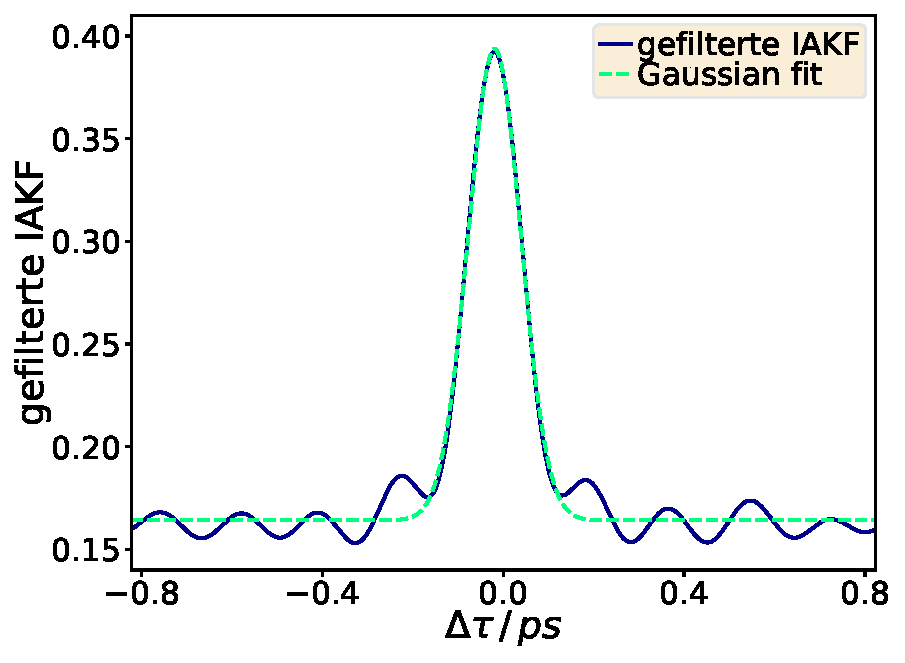
\includegraphics[width=0.65\textwidth]{Gauss.pdf}
    \caption{\label{fig:gauss}Die gefilterte IAKF vergleichend zu der angefitteten Gaußfunktion (gestrichelt).}
\end{figure}\FloatBarrier
Wie in der vorbereitenden Frage \ref{subsec:FZV1} behandelt, ergibt sich 
das Zeit-Bandbreiten-Produkt der Autokorrelation aus dem Produkt der Pulsbreite 
der gemessenen Leistung ($\left\vert a(t) \right\vert^{2}$) und der spektralen Breite. 
Der herausgefilterte relevante Beitrag der IAKF erfüllt folgende Proportionalität
\begin{equation}
    \langle P_{\text{Sig}}(t) \rangle \,\sim \int\,dt\,\left\vert a(t) \right\vert^{2}\left\vert a(t-\Delta\tau)\right\vert^{2}, 
\end{equation}
woraus mit Annahme eines gaußförmigen Pulses folgt, dass die Breite der IAKF $\Delta t_{\text{IAKF}}$ folgendermaßen 
mit der Pulsbreite $\Delta t_{\text{FWHM}}$ zusammenhängt
\begin{equation}
    \Delta t_{\text{FWHM}} = \frac{1}{\sqrt{2}}\Delta t_{\text{IAKF}}.
\end{equation}
Die Breite der IAKF errechnet sich aus Varianz der gefitteten Gaußfunktion zu
\begin{equation}
    \Delta t_{\text{IAKF}} = 2\sqrt{2\ln(2)}\,\sigma,
\end{equation}
woraus wir eine Bestimmungsgleichung für die Pulsbreite, sowie deren Fehler erhalten
\begin{align}
    \Delta t_{\text{FWHM}} &= \frac{1}{\sqrt{2}}2\sqrt{2\ln(2)}\,\sigma \\
    &= 2\sqrt{\ln(2)}\,\sigma \\
    s_{\Delta t_{\text{FWHM}}} &= \left\vert\frac{\partial \Delta t_{\text{FWHM}}}{\partial \sigma}\right\vert s_{\sigma} \\
    &= 2\sqrt{\ln(2)}\,s_{\sigma}.
\end{align}
Einsetzen der Werte resultiert in folgendem Ergebnis
\begin{equation}
    \Delta t_{\text{FWHM}} = (0,097 \pm 0,005)\,\si{ps}.
\end{equation}
Mit Gl.~\eqref{eq:spektrale} folgt für das Zeit-Bandbreiten-Produkt
\begin{equation}
    \fbox{$\Delta t_{\text{FWHM}}\Delta \nu_{\text{FWHM}} = (0,93 \pm 0,07)$}.
\end{equation}
Das Zeit-Bandbreiten-Produkt ist wie erwartet größer als das eines idealen Gaußpulses (siehe Abschnitt \ref{subsec:FZV1}),
da das optische Spektrum des Lasers deutlich von dieser idealen Form abweicht. Dennoch scheint das Ergebnis sinnvoll, da 
der errechnete Wert im gleiche Bereich liegt. \\
Insgesamt können wir in diesem Versuchsteil schöne und sinnvolle Ergebnisse produzieren, was darauf hindeutet, dass der 
Messaufbau gut war und die Messung richtig funktioniert hat. Zudem sind die Werte kompatibel mit den theoretischen 
Erwartungen, was die Richtigkeit stützt. \\
